\section{Einleitung}
\label{sec:einleitung}
Das vorliegende Dokument ist die Ausarbeitung der Aufgabenstellung für die Klausur zur Lehrveranstaltung \emph{Qualtity Engineering}. Als Softwareprodukt wird die Softwarelösung \emph{clever\textbf{cure}} des Unternehmens \hyperlink{http://www.curecomp.com/}{\emph{curecomp Software Services GmbH}} gewählt, die eine Softwarelösung für den Bereich \emph{Supplier Relationship Management (SRM)} ist. 
\newline
\newline
\emph{SRM} umfasst die zentrale Steuerung und Planung der Beziehungen eines Unternehmens zu seinen Lieferanten, wobei erreicht werden soll, dass die Lieferanten eng an das Unternehmen angebunden werden und dass das Vertrauen zwischen den Kunden und seinen Lieferanten gestärkt wird. Ebenfalls ist es ein Ziel einen hohen Automatisierungsgrad zu erreichen, um dadurch die Einkaufsprozesse des Kunden und die Dispositionsprozesse der Lieferanten zu optimieren.  
\newline
\newline
Die Softwarelösung \emph{clever\textbf{cure}} stellt eine zentrale Schnittstelle zwischen den Kunden und den Lieferanten zur Verfügung und versucht einen hohen Automatisierungsgrad zu erreichen, um die Einkaufsprozesse der Kunden und auch die Dispositionsprozesse der Lieferanten zu optimieren. Ein Hauptziel ist es die Einkaufsprozesse und Dispositionsprozesse ohne Medienbruch durchführen zu können.

\begin{figure}[h]
	\centering
	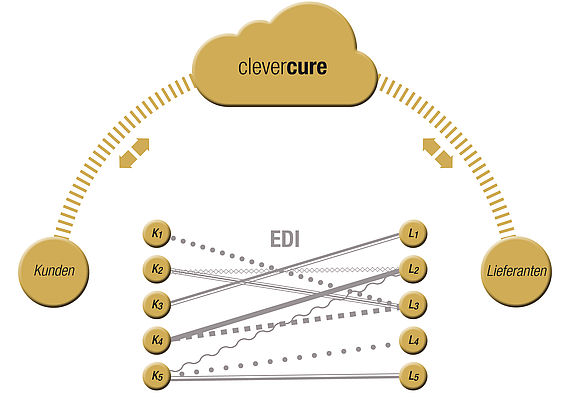
\includegraphics[scale=0.6]{\imageDir/clevercure_principle.jpg}
	\caption{Das Prinzip von \emph{clever\textbf{cure}}}
	\label{fig:clevercure-principle}
\end{figure}
\ \newline
Bei der Softwarelösung \emph{clever\textbf{cure}} handelt es sich aus der Sicht der Kunden und der Lieferanten um eine \emph{Cloud}basierte Softwarelösung, die als \emph{Software as a Service (SAAS)} zur verfügung gestellt wird.
\newpage

Da Lieferanten auf verschiedene Art und Weise arbeiten wie z.B. kleine Unternehmen mit \emph{Excel} und große Unternehmen mit z.B. \emph{SAP} werden einerseits eine Webanwendung und andererseits eine Schnittstellenanwendung benötigt, womit gewährleistet wird, dass die Kunden mit all ihren Lieferanten \emph{SRM} betreiben können.
\newline
\newline  
Aus dem oben genannten Gründen ist die Softwarelösung \emph{clever\textbf{cure}} auf die folgend beschriebenen drei Anwendungen aufgeteilt.
\begin{itemize}
	\item\emph{clever\textbf{web}} ist die Webanwendung, über welche die Kunden und die Lieferanten operative wie auch strategische Aufgaben durchführen können,
	\item\emph{clever\textbf{interface}} ist die Schnittstellenanwendung, über welche die Kunden und die Lieferanten mit ihren \emph{ERP}-System angebunden sind und
	\item\emph{clever\textbf{document}} ist das Dokumentenmanagementsystem, welches alle anfallenden Dokumente für die Kunden und die Lieferanten verwaltet. 
\end{itemize}

